\section{Experimental evidence}\label{sec:results}
\subsection{Controlled failures with known score mechanisms}
We sampled $Y\sim{\rm Bernoulli}(\pi)$ and $X\mid Y=y\sim N((2y-1)d/2,1)$. The grid crosses $n\in\{40,80,160,320,640\}$, $\pi\in\{0.3,0.5,0.7\}$, $d\in\{0.5,1,2\}$ and three seeds (17, 29, 43). Each of the 135 cells contains 1,000 repetitions. First, $s=X+1$ moves the zero decision but preserves ranks and the family of static threshold decisions. Next, $0.2s$ preserves the sign of $s$ while changing the probability obtained by applying the sigmoid. In a separate intervention, $s+\epsilon$, $\epsilon\sim N(0,1)$ independent, corrupts ordering. Default BA, oracle BA, AUC and expected calibration error (ECE) are computed on each simulated sample.

\begin{figure*}[t]
\centering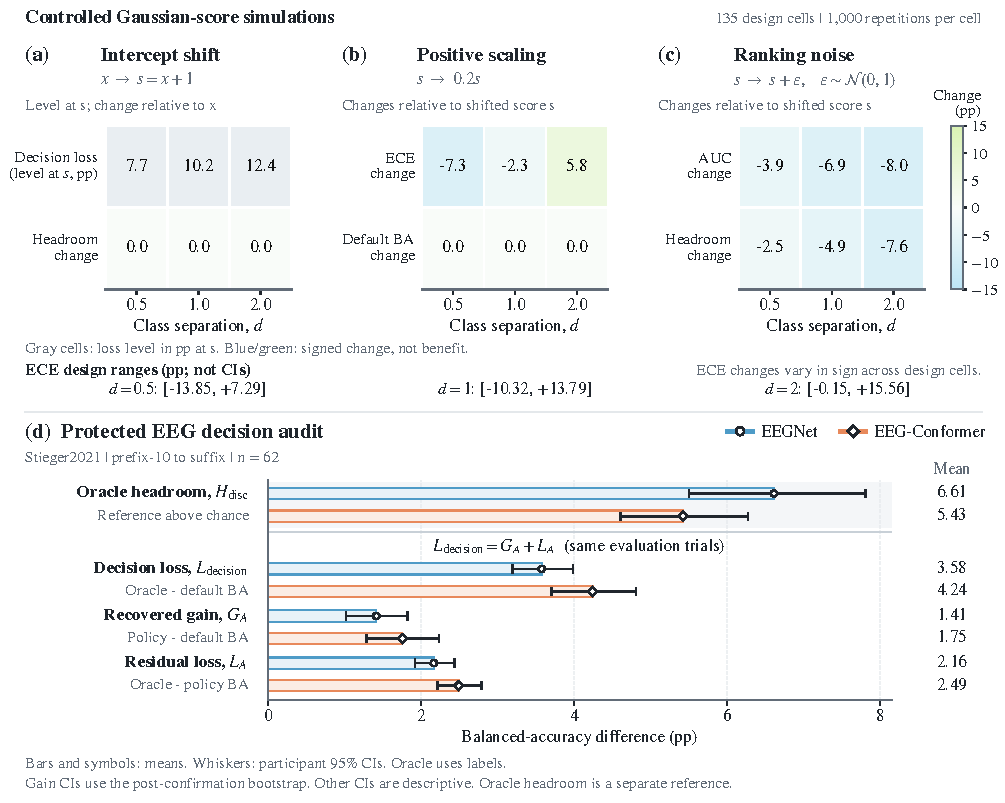
\includegraphics{figures/figure2_construct_protected_audit.pdf}
\caption{Known score interventions and the protected Stieger decomposition. (a)--(c) Each cell averages 45 design settings at the indicated class separation. The ECE ranges beneath the panels give the smallest and largest cell means at each separation. Intercept-shift loss is a level at the shifted score. Scaling and noise are changes relative to that score. (d) The 62 Stieger participants contribute model-averaged estimates on trials 11 onward. The whiskers give marginal 95\% participant intervals. The gain uses the post-confirmation participant bootstrap. The other component intervals are descriptive.}\label{fig:construct}
\end{figure*}

Figure~\ref{fig:construct}(a)--(c) distinguishes the changes in decisions, probability calibration and ranking. The intercept preserved empirical oracle headroom exactly but left 7.71--12.45 points of default decision loss on average across the three separation levels. Compression gave exactly the same default decisions in every repetition. Its mean ECE change was $-7.32$, $-2.31$ and $+5.85$ points as $d$ increased. Independent noise lowered both AUC and headroom at all three levels. The largest tested accounting residual was zero. A separate paired class-stratified normal interval targeted population BA loss between the \emph{known} Gaussian-optimal threshold and zero. Its lowest coverage across cells with $n\geq160$ was 92.8\%, above the 92\% gate and below nominal 95\%. This check concerns that interval and known threshold. EEG sampling uncertainty and fitted-oracle optimism require separate evidence.

A balanced prior also leaves the threshold unidentified. Consider equiprobable scores $-3,-2,\ldots,4$ and the following two monotone right-class probabilities, in percent, in score order. World A has $(1,1,49,49,60,60,80,100)$ and world B has $(0,40,55,55,60,60,65,65)$. Both have prior 0.5. Enumerating the nine threshold splits gives optimal BA of 0.75 for a threshold in $(0,1]$ in A and 0.65 in $(-2,-1]$ in B. The score marginal and prior available to the policy are identical. This construction limits what can be inferred from observed success of a median rule.

\subsection{Discovery and locked confirmation}
\begin{figure}[t]
\centering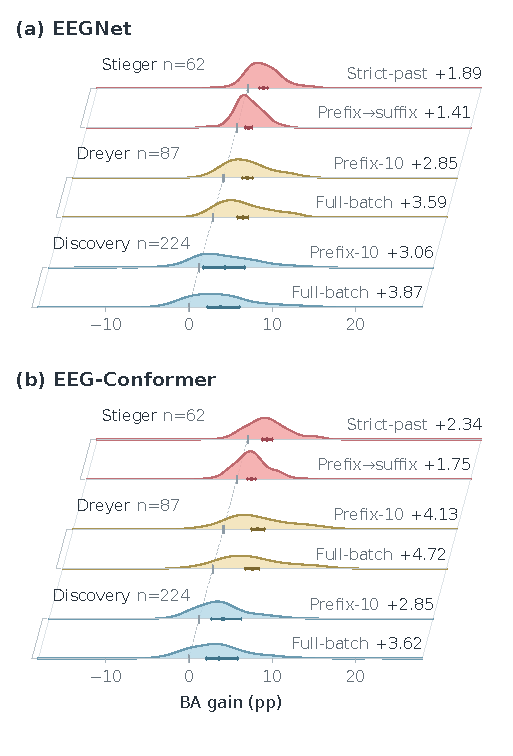
\includegraphics{figures/figure2_cross_cohort_forest.pdf}
\caption{Prior-quantile gain over the matched default decision. Dots show mean gains. Bars give 95\% bootstrap intervals from the discovery and Dreyer analyses and the post-confirmation participant bootstrap for Stieger. Ridges show Gaussian densities of participant gains on a shared scale with Scott bandwidths. Depth separates endpoints. Within a cohort the same people contribute to each row. Historical prefix and batch score the complete record. Stieger prefix and strict-past score trials 11 onward.}\label{fig:cohorts}
\end{figure}

In Fig.~\ref{fig:cohorts}, the discovery prefix-ten gains were 3.06 [0.50, 5.42] and 2.85 [1.43, 5.01] BA points for EEGNet and the Conformer, respectively. Full-batch gains were 3.87 [2.23, 6.08] and 3.62 [2.13, 5.85]. Discovery intervals resample datasets, protocols and participants hierarchically. Dreyer and Stieger intervals resample participants after source and seed averaging. After aggregation within participants, historical prefix ten gave a negative gain for 20.5\% of EEGNet and 19.2\% of Conformer participants in discovery. The fifth percentiles of gain were $-2.00$ and $-1.71$ points. The archived discovery tail non-degradation criterion failed. Discovery stores probabilities, some saturated, so converting them back to logits cannot recover the original score ordering at the extremes. Its decision results can be used at their recorded precision.

On Dreyer, prefix-ten gains were 2.85 [2.29, 3.45] and 4.13 [3.36, 4.91] points. Complete-batch gains were 3.59 [2.98, 4.24] and 4.72 [3.88, 5.56]. Default BA was 55.33\% for EEGNet and 51.66\% for the Conformer. Historical prefix ten retained 79.3\% and 87.3\%, respectively, of each model family's complete-batch gain. At the historical prefix endpoint, 11.5\% and 9.2\% of participants respectively lost accuracy. Both backbones met the secondary 75\% recovery criterion and the complete-batch magnitude and interval criteria. However, mean participant AUC was 0.620 and 0.585 against a required 0.60. Changing raw-BN to raw-GroupNorm gained 5.02 and 1.55 points against a two-point criterion. Only EEGNet met both of these primary gates. Worst-participant BA under complete-batch repair fell from 47.14\% to 47.03\% for EEGNet and from 49.81\% to 47.06\% for the Conformer. A lower minimum describes the cohort tail and need not refer to the same individual before and after repair.

\subsection{Protected external endpoint}
\begin{table}[t]
\caption{External cohort, 62 participants. Top rows give absolute percentages on the protected suffix for prefix ten. Bottom rows give prior-quantile gains in points versus the default on each rule's evaluation rows (Table~\ref{tab:contracts}). Brackets give marginal 95\% participant intervals. Gain intervals use the post-confirmation bootstrap.}\label{tab:primary}
\centering\small\setlength{\tabcolsep}{4pt}\begin{tabular}{@{}lrr@{}}\toprule
Protected measure (\%) & EEGNet & Conformer \\\midrule
Default BA & 53.04 [52.26, 53.90] & 51.18 [50.85, 51.55] \\
Quantile BA & 54.45 [53.38, 55.60] & 52.93 [52.19, 53.67] \\
Rank AUC & 57.02 [55.39, 58.75] & 54.95 [53.80, 56.11] \\
Oracle BA & 56.61 [55.50, 57.81] & 55.43 [54.60, 56.28] \\
\midrule Gain by access (pp) & EEGNet & Conformer \\\midrule
Fixed prefix 10 & 1.41 [1.01, 1.82] & 1.75 [1.28, 2.23] \\
Strict past & 1.89 [1.40, 2.39] & 2.34 [1.75, 2.95] \\
Session forward & 1.63 [1.14, 2.11] & 2.07 [1.50, 2.66] \\
Complete batch & 1.89 [1.40, 2.40] & 2.42 [1.84, 3.03] \\
\bottomrule\end{tabular}
\end{table}

The frozen external models produced 30 score streams over the same 69,628 distinct Stieger trials. The protected median sees ten unlabeled scores per participant and predicts on trials 11 onward. Table~\ref{tab:primary} pairs each gain with its default, its final accuracy and the BA attainable with suffix labels. Moving the threshold raised BA from 53.04\% to 54.45\% for EEGNet and from 51.18\% to 52.93\% for the Conformer. The participant-bootstrap intervals for gains of 1.41 and 1.75 points both exclude zero. Both point estimates fall short of the two-point magnitude criterion. The Conformer interval crosses two points, but its point estimate determines the branch. The protected conclusion remains \emph{mixed}.

AUC exceeds chance, yet even the fitted static oracle attains only 56.61\% and 55.43\% BA on average. Figure~\ref{fig:construct}(d) places these measurements on a common BA-difference scale. The estimated default decision loss is 3.58 and 4.24 points. After prefix fitting, 2.16 and 2.49 points remain between the policy and the label-informed static reference. The accounting relation holds before rounding. Separate marginal intervals for its terms need not add. This combination of working threshold repair and limited absolute discrimination constrains the practical interpretation.

\begin{table*}[!t]
\caption{Changing fitting budget and evaluation start. Historical moving-suffix columns show mean BA gains in points. The post-hoc common suffix includes marginal 95\% descriptive intervals, using the same 10,000 participant draws across budgets. Each pair lists EEGNet then Conformer.}\label{tab:common}
\centering\small\begin{tabular}{@{}lrrrrrr@{}}\toprule
$k$ & Fixed, Net & Fixed, Conf. & Past, Net & Past, Conf. & Common, EEGNet & Common, Conformer \\\midrule
5 & 1.22 & 1.70 & 1.88 & 2.34 & 1.19 [0.85, 1.54] & 1.67 [1.23, 2.12] \\
10 & 1.41 & 1.75 & 1.89 & 2.34 & 1.38 [0.98, 1.78] & 1.72 [1.24, 2.20] \\
20 & 1.51 & 1.90 & 1.88 & 2.34 & 1.50 [1.07, 1.92] & 1.87 [1.36, 2.39] \\
50 & 1.59 & 1.95 & 1.86 & 2.33 & 1.59 [1.13, 2.04] & 1.95 [1.42, 2.46] \\
\bottomrule\end{tabular}
\end{table*}

\subsection{Access windows and the cost of moving the test set}
Strict-past refitting yielded 1.89 and 2.34 points on the same trials 11 onward as the fixed-prefix rule (Table~\ref{tab:primary}). Both the amount of available past data and the opportunity to update change. A first-session fit is held fixed on subsequent sessions, so it tests transfer across acquisitions. The full-batch threshold reads future scores and evaluates early trials too. Under strict-past updating, 19 of 930 EEGNet and 28 of 930 Conformer participant--model rows exceeded their in-sample static oracle, producing a negative signed residual. No participant had a negative mean residual after model averaging. A larger cohort mean in one of these rows alone provides no chronological comparison of deployable policies.

In the historical $k$ sweep, fixed-prefix accuracy is evaluated on $k+1,\ldots,n$. Changing $k$ alters both the fit and the test set. In the corresponding strict-past sweep, increasing $k$ only postpones the evaluation start. The prediction for a shared trial still uses all its predecessors. To isolate fitting budget, the post-hoc analysis fixes the evaluation rows at $51,\ldots,n$ for $k=5,10,20,50$. It requires the same eligible participants and 15 models per backbone at every budget. Scores between the fit and trial 51 are unavailable to the fitted threshold. The common-window design was specified after the historical study and before this comparison was computed.

All 62 participants contributed the same 66,528 distinct suffix trials under every budget. From five to fifty available scores the mean gain changed from 1.19 to 1.59 points for EEGNet and from 1.67 to 1.95 for EEG-Conformer. These estimates describe budget sensitivity on a fixed sample. They do not select a deployment budget or revise the protected gate.

Table~\ref{tab:common} reports all four budgets, including those between the two extremes. For example, the protected $k=10$ and the common-window $k=10$ use identical fitted thresholds. Their different gains measure the effect of scoring different rows. Neither the moving-window sequence nor the marginal intervals constitute a paired test for an optimal $k$.

\subsection{Access-matched controls and their adverse outcomes}
A source-only Youden threshold gained 0.68 points [0.49, 0.89] for EEGNet and 0.84 [0.60, 1.09] for the Conformer on the protected suffix. Source intercept and source Platt moved the decision less, yielding mean gains between 0.16 and 0.30 points. Positive temperature left every zero-logit decision unchanged. For the paired cutoff comparison on the same Platt-v2 fit, changing the source cutoff from 0.5 to $\pi_s$ changed gain from 0.23 to 0.27 points for EEGNet and from 0.30 to 0.27 for the Conformer. Access to validation labels and the choice of utility both matter even before a target score is observed.

\begin{table}[t]
\caption{Protected suffix by policy. The last two columns count participants with negative gain and gain below $-2$ points, respectively, out of 62, after averaging over models. Source Platt is source-only. The remaining rules read the first ten target scores. EM and BBSE additionally use the fitted source map.}\label{tab:policies}
\centering\footnotesize\begin{tabular}{@{}lrrrr@{}}\toprule
Backbone & Policy & Gain [95\% CI] & $<0$ & $<-2$ \\\midrule
EEGNet & Source Platt & 0.23 [0.13, 0.32] & 20 & 0 \\
EEGNet & Prior quantile & 1.41 [1.01, 1.82] & 9 & 1 \\
EEGNet & Platt--EM & -2.48 [-3.12, -1.89] & 55 & 29 \\
EEGNet & Ridge BBSE & -2.33 [-2.92, -1.76] & 55 & 27 \\
Conformer & Source Platt & 0.30 [0.16, 0.46] & 19 & 0 \\
Conformer & Prior quantile & 1.75 [1.28, 2.23] & 11 & 1 \\
Conformer & Platt--EM & -1.00 [-1.29, -0.75] & 52 & 11 \\
Conformer & Ridge BBSE & -1.01 [-1.28, -0.76] & 53 & 11 \\
\bottomrule\end{tabular}
\end{table}

Table~\ref{tab:policies} shows the contrast within the protected target window. Both posterior-at-0.5 corrections reduced participant-averaged BA for most participants. Changing the Ridge BBSE shrinkage over the prespecified values retained negative mean gains. In particular, EEGNet's EM rule lost more than two points for 29 of 62 participants. The shared ten-score budget alone does not determine the direction of a change. Prior estimation, source calibration and the decision objective can all affect these results. The observed deficits cannot identify which assumption failed.

Target-signal methods can also change the score ranking. In historical paired comparisons against each corresponding frozen raw-BN checkpoint (224 participants), full-signal AdaBN gained 5.78 EEGNet and 4.30 Conformer points. Sequential TENT changed BA by $-4.86$ and $-0.65$ points, and T3A by $-1.12$ and $-0.97$~\cite{wang2021tent,iwasawa2021}. The official T-TIME port used a distinct matched baseline, its IEA-only component~\cite{li2024ttime}. Aggregating 2,688 paired participant-run differences within the 224 participants gave $-2.38$ BA points and $-4.58$ AUC points. A ranking change is possible in this block. These runs use historical target signals and their own matched baselines, which precludes a performance ordering with the Stieger score-only policies.
